\documentclass[letterpaper,12pt]{report}
\usepackage{McECEThesis}
\usepackage{amsmath}
\usepackage{amsfonts}
\usepackage{mathrsfs}
\usepackage[dvips]{graphicx}
\begin{document}
\author{Nicholas Esterer}
\title{Elements of Source Separation}
\maketitle
\tableofcontents

\section{Introduction}
In signal processing, a common task is the separation of a signal with known
deterministic or statistical characteristics from another. This task has been
well studied \cite{kay1993fundamentals} \cite{hayes2009statistical}
\cite{poor2013introduction} and works well for problems of digital communication
or object detection where these characteristics are well known. In digital
communication, the signals and techniques to transmit them are often optimized
by the designer to make them robust to corruption or interference. The designers
of vehicles usually design them to be predictable and reliable and so their
positions in time will reflect this. In this thesis we tacle a more difficult
problem, that of the separation of a mixture of acoustic signals. The nature of
these signals is different in that their design criteria are either
mostly unknown or fundamentally different. For example, musical instruments are
designed to have desirable acoustic properties which are generally subjective.
As an example of one of the complications, the choirs of the orchestra are sets
of instruments actually designed to blend well; to sound as one instrument.
Ironically, it is this criterion that we use to guide the source separation
techniques described in the following.

\section{Methodology}
Perceptual studies have shown that sounds modulated synchronously in amplitude
or frequency are heard as one sound, whereas asynchronously modulated sounds are
heard as distinct \cite{mcadams1989segregation} \cite{marin1991segregation}.
Here we define the modulation of parameters $\theta_i$ and $\theta_j$ as being
synchronous if they are given as functions of time, $\theta_i=f_i(t)$ and
$\theta_j=f_j(t)$ and there is an affine transform $\mathscr{A}$ such that
$\mathscr{A}\{f_i\}(t) \approx A f_j(t) + B$ where $A$ and $B$ are constants
that do not vary with time (at least for the time that we observe the signal).
If we can accurately measure these parameters and they are typical of the sounds
we are trying to separate, then we can design techniques to reliably separate
these sounds from acoustic mixtures. This involves picking those parameters
classified as belonging to the same sound, discarding the rest, and
resynthesizing from these parameters. The task of audio source separation
therefore comprises the following tasks:

\begin{itemize}
    \item
        Decide on a signal model for the sound of interest, with parameters that
        can be estimated and that are similar for similar sounds.
    \item
        Estimate the signal parameters.
    \item
        Classify the parameters and group them as sets of parameters coming from
        the same source: the sound of interest.
    \item
        Choose a group of parameters and synthesize the separated signal from
        them.
\end{itemize}

This thesis describes various approaches to the above tasks and utilises some of
them in source separation experiments.

\section{Signal Modeling}

\subsection{Time-Frequency Representations}

As most musical instruments are resonating media and excited resonating media
are well described as linear time-invariant (LTI) auto-regressive (AR)
structures, popular models of musical audio are some variation of this
description.
% Need citation

An LTI auto-regressive structure is a signal that can be desribed using the
following \textit{difference equation}:

\begin{equation}
    x(n) = \sum_{k=1}^{K} a_k x(n-k) + b_0 v(n)
\end{equation}

Here $x$ is the output of the system (what is heard or measured) and $v$ is the
input. $K$ is the order of the model. Both are general functions of time which,
in the case of properly sampled digital audio, can be considered at times $n \in
\mathbb{Z}$ without any loss of information. $a_k,b_0 \in \mathbb{C}$ and are
constants. Casually (no pun intended) you can think of the output of the system
at time $n$ as being a linear combination of past outputs, plus some of the
scaled input.

AR structures are excited in various ways: some are bowed, others struck, etc.
To characterize the above structure we excite it with a simple signal, the
\textit{delta function}

\begin{equation}
    \delta(n) = \begin{cases}
        1 & n=0\\
        0 & \text{otherwise}
    \end{cases}
\end{equation}

This delta function input will yield its \textit{impulse
response} from which we can derive many properties of the AR structure.

As an example take the case where $K=1$ and $a_1 = r \exp(j\omega)$, 
$r\text{,}\omega \in \mathbb{R}$, $|r|<1$ (recall that $j=\sqrt{-1}$ and is
called the \textit{imaginary number}). Then the difference equation is

\begin{equation}
    x(n) = r \exp(j\omega) x(n-1) + v(n)
\end{equation}

Exciting this with the delta function we get
\begin{equation}
    \begin{array}{c}
        x(0) = 1 \\
        x(1) = r \exp(j\omega) \\
        x(n) = r^n \exp(j\omega n)
    \end{array}
\end{equation}

which is a complex exponential starting at $n=0$ and periodic in
$n_T=\frac{2\pi}{\omega}$ multiplied by the real-valued
exponential $r^n$. In other words, the output is a damped exponential. From this
it is not hard to see that if we can estimate the coefficients $a_k$, we can
then know the frequencies, amplitudes and damping factors of the sinusoids that
are output when this structure is excited by an impulse (the delta function).
This technique is presented as a motivation for the following techniques and is
not pursued here. The interested reader is referred to \cite{makhoul1975linear}
for more information.

An alternative method for determining the frequencies and amplitudes of
sinusoids in mixture is to take the inner-product of the signal with a complex
exponential of known frequency and see what you get

\begin{equation}
    X(\omega) = \sum_{n=-\infty}^{\infty} x(n) \exp(-j \omega n)
\end{equation}

The function $X(\omega)$ will be large if $x(n)$ contains a complex exponential of
frequency $\omega$ and small if it doesn't, effectively indicating which
sinusoidal functions are present in the signal. This transformation of a signal
as a function of time $n$ into one as a function of frequency $\omega$ is known
as the \textit{Discrete-time Fourier Transform} (DTFT). 

To create a variety of pitches and timbres, typically the media of musical
instruments are not static, but vary in time. That means the sets of sinusoids
describing the state of the media and its excitation also change in time. To
account for this we consider many small intervals of signal where we assume its
characteristics are roughly static. We can then piece these time-intervals
together afterwards to get a description of the signal in both time and
frequency. To do this, we multiply the signal by a window $w$ which makes the signal
0 outside of the interval of interest. We then test what sinusoids with
frequencies $\omega$ are present at different times $\tau$, giving a function of
two variables

\begin{equation}
    X(\tau,\omega) = \sum_{n=-\infty}^{\infty} x(n) w(n - \tau) \exp(-j \omega n)
\end{equation}

This transformation of a signal of time $n$ in to one of time $\tau$ and
frequency $\omega$ is known as the \textit{Discrete-time Short-time Fourier
Transform} (DTSTFT).

\subsection{Polynomial Phase Models}

The DTFT and DTSTFT are very useful because they are invertible
\cite{portnoff1976implementation} and fast algorithms exist for their 
computation by digital computer \cite{van1992computational}. If the presence of
a sinusoid is determined, e.g., by finding $\tau^{\ast}$ and $\omega^{\ast}$ such that
$X$ is maximized, that signal can be removed or altered easily.

One drawback of these transforms is they only project onto sinusoidal functions
of linear phase, i.e., functions of constant frequency. In general, musical
signals are not linear combinations of sinusoids of constant frequency
(consider, for example, vibrato). We could decide to project onto a different
family of functions and considerable effort has been devoted to finding
alternatives (see \cite{kereliuk2011sparse} for a review). In the case of
musical signals, however, we have some prior information and can make certain
assumptions about the underlying functions.

\subsubsection{Sinusoidal Representations}

Many musical acoustic signals are quasi-harmonic, meaning that they consist of a
sum of sinusoids whose frequencies are roughly integer multiples of a
fundamental frequency. For these kinds of signals, most of the energy can be
attributed to sinusoids and so, if we neglect the noisy part of the signal, the
signal can be described by a small number of sinusoids with slowly varying
amplitude and phase, plus some noise. The model is

\begin{equation}
    x(n)=\sum_{p=1}^{P} A_p(n) \exp(j \phi_p(n)) + \varepsilon
\end{equation}

where $\varepsilon \sim \mathcal{N}(0,\sigma)$ and $A_p \in \mathbb{R}$ and
$\phi_p \mathbb{R}$ are functions of amplitude and phase respectively. In the
following, we consider equivalent sinusoidal mixtures of complex-valued
polynomial phase exponentials
\begin{equation}
    x(n)=\sum_{p=1}^{P} \exp(\mathcal{P}_p(n)) + \varepsilon
\end{equation}
where
\begin{equation}
    \mathcal{P}_p(n) = \sum_{q=0}^{Q} c_q n^{q}
\end{equation}

and $c_q \in \mathbb{C}$.

The sum-of-sinusoids model of McAulay and Quatieri estimates these coefficients
in an indirect way \cite{mcaulay1986speech}. Given two local maxima of the
DTSTFT $X(\tau_0,\omega_0)$ and $X(\tau_1,\omega_1)$, where $H = \tau_1 -
\tau_0$ we can conjecture a cubic
polynomial phase function for the imaginary part of the phase argument

\begin{equation}
    \tilde{\phi}(n) = c_3 (n-\tau_0)^3 + c_2 (n-\tau_0)^2 + c_1 (n-\tau_0) + c_0
\end{equation}

By noting that we have 2 measurements of the phase and frequency,
$\angle\{X(\tau_0,\omega_0)\}$ and $\angle\{X(\tau_1,\omega_1)\}$, and the frequency
is the derivative of the phase, we can solve for the coefficients of the
polynomial phase function using the following linear system of equations
\begin{equation}
    \begin{pmatrix}
        0   & 0     & 0 & 1 \\
        H^3 & H^2   & H & 1 \\
        0   & 0     & 1 & 0 \\
        3 H^2 & 2 H & 1 & 0
    \end{pmatrix}
    \begin{pmatrix}
        \Im\{c_3\} \\
        \Im\{c_2\} \\
        \Im\{c_1\} \\
        \Im\{c_0\}
    \end{pmatrix}
    =
    \begin{pmatrix}
        \angle\{X(\tau_0,\omega_0)\} \\
        \angle\{X(\tau_1,\omega_1)\} + 2 \pi M \\
        \omega_0 \\
        \omega_1        
    \end{pmatrix}
\end{equation}
and choosing $M$ so that
\begin{equation}
    \int_{0}^{H}(\tilde{\phi}^{\prime\prime}(t))^{2}dt
\end{equation}
is minimized.

As only two measurements of the amplitude of the sinusoid are available,
$|X(\tau_0,\omega_0)|$ and $|X(\tau_1,\omega_1)|$, the coefficients
$c_3$ and $c_2$ are purely imaginary and the real parts of $c_1$ and $c_0$ are
determined as
\begin{equation}
    \begin{pmatrix}
        0 & 1 \\
        H & 1
    \end{pmatrix}
    \begin{pmatrix}
        \Re\{c_1\} \\
        \Re\{C_0\}
    \end{pmatrix}
    =
    \begin{pmatrix}
        \log(|X(\tau_0,\omega_0)|) \\
        \log(|X(\tau_1,\omega_1)|)
    \end{pmatrix}
\end{equation}

\subsubsection{Polynomial phase parameter estimation}

More recently a set of techniques have been developed that use some combination
of derivatives of the analysis window $w$ or the signal $x$ to estimate the
polynomial coefficients directly \cite{hamilton2011non}. For this thesis we will
only consider a technique that does not estimate derivatives of the signal and
only requires a once-differentiable analysis window as it is relatively easy to
implement and suits our purposes.

The following is adapted from \cite{betser2009sinusoidal}. Consider the inner
product of the signal $x(n) = \exp(\mathcal{P}_p(n)) $ and a
known analysis \textit{atom} $\psi(n)$
\[
    f(n) = \left\langle x,\psi \right\rangle =
    \int_{-\infty}^{\infty}x(n)\overline{\psi}(n)dn
\]
Differentiating with respect to $n$ we obtain
\[
    \frac{df}{dn}(n) = \frac{dx}{dn}(n)\overline{\psi}(n)
    + x(n)\frac{d\overline{\psi}}{dn}(n)
    = \left( \sum_{q=1}^{Q} q c_q n^{q-1} \right) x(n)\overline{\psi}(n)
    + x(n)\frac{d\overline{\psi}}{dn}(n)
\]

If $\psi(t)$ is 0 outside of some interval $n \in [-T,T]$ then
\[
    \int_{-T}^{T} \frac{dx}{dn}(n)\overline{\psi}(n) dn
    = \sum_{q=1}^{Q} q c_q \int_{-T}^{T} n^{q-1} x(n) \overline{\psi}(n) dn
    + \left\langle x, \frac{d\overline{\psi}}{dn} \right\rangle = 0
\]
which after rearranging is
\[ 
    \sum_{q=1}^{Q} q c_q 
    \left\langle n^{q-1} x(n) , \overline{\psi}(n) dn \right\rangle
    = -\left\langle x, \frac{d\overline{\psi}}{dn} \right\rangle
\]
From this we can see that to estimate the coefficients $c_q$, $ 1 \leq q \leq Q
$ we simply need $R$ atoms with $R \geq Q$ to solve the linear system of
equations
\[ 
    \sum_{q=1}^{Q} q c_q 
    \left\langle n^{q-1} x(n) , \overline{\psi_{r}}(n) dn \right\rangle
    = -\left\langle x, \frac{d\overline{\psi_{r}}}{dn} \right\rangle
\]
for $1 \leq r \leq R$. Estimation of the coefficients of a phase polynomial
using this method is known as the \textit{Distribution Derivative Method (DDM)}.

\subsubsection{The choice of atom $\psi$}

As we are dealing with mixtures of sinusoids of small bandwidth, in addition to
the finite time support constraint, we desire atoms whose inner-product is only
significant within a finite bandwidth of interest. To construct these atoms, we
multiply the Fourier atom by the window $w$
\[
    \psi_{\tau,\omega}^{\mathcal{F}_{w}}(n) = w(n-\tau) \exp(-j\omega(n-\tau))
\]

A good overview of different windows and their properties is given in
\cite{harris1978use}. We require that the window be at least
once-differentiable and zero outside of a certain interval, therefore, somewhat
informally, we require
\[
    \lim_{n \rightarrow T} \psi(n) = \psi(T) = 0
\]
The \textit{Hann} window possesses this property
\[
    w_{h}(n) = \begin{cases}
        0.5 + 0.5 \cos \left( \frac{n}{T}\pi \right) & -T \leq n \leq T \\
        0 & \text{otherwise}
    \end{cases}
\]

The Hann window is a member of a class of windows constructed by summing scaled
harmonically related cosine functions, subject to the constraint that the
scaling coefficients sum to 1 so that the window have a value of 1 at $n=0$.
Letting $T=N/2$, where $N$ is the length of the window
\[
    w(n) = \begin{cases}
        \sum_{m=0}^{M-1}a_{m}\cos \left( \frac{2\pi}{N}mn \right) & -\frac{N}{2} \leq n
        \leq \frac{N}{2} \\
        0 & \text{otherwise}
    \end{cases}
\]
With $M=2$ and $a_0 = a_1 = 0.5$, we have the Hann window. The
\textit{Blackman-Harris} family of windows are also sum-of-cosine windows. For
these windows, optimization techniques were used to search for coefficients
giving optimum properties, such as minimum height of the highest side-lobe
(maximum out-of-band rejection) \cite{rabiner1970approach}. The 4-term window
whose coefficients $a$ are listed in table~\ref{tab:opt_blackman} has a maximum
side-lobe level of 92 dB, lower than the quantization noise of a 16-bit linear
pulse code modulated signal. This window has a very large main-lobe which means
two sinusoids of similar frequency will be difficult to resolve. Furthermore,
the window has a discontinuity at its boundaries, e.g.,
$w \left( \frac{N}{2} \right) \neq 0$ and is not once-differentiable.

To find a window with properties similar to the 4-term Blackman-Harris window
but without a discontinuity, we solve the optimization problem
\[
        \min||a-\tilde{a}||_2 \\
\]
subject to
\[
        w_{\tilde{a}} \left( \frac{N}{2} \right)
            = w_{\tilde{a}} \left( \frac{-N}{2} \right) = 0
\]
\[
        \sum_{m}^{M-1} a_{m} = 1
\]
where
\[
    w_{\tilde{a}}(n) = \begin{cases}
        \sum_{m=0}^{M-1}\tilde{a}_{m}\cos \left( \frac{2\pi}{N}mn \right) & -\frac{N}{2} \leq n
        \leq \frac{N}{2} \\
        0 & \text{otherwise}
    \end{cases}
\]
The solution $\tilde{a}^{\ast}$ is given in Table~\ref{tab:opt_blackman} and
plots are given in Figure~\ref{plot:opt_blackman}. This window will be referred
to as the $\mathcal{C}^{1}$ 4-Term Blackman-Harris window.

\begin{table}
    \caption{\label{tab:opt_blackman}}
    \begin{center}
        \begin{tabular}{l c c c c }
            Window & $a_0$ & $a_1$ & $a_2$ & $a_3$ \\
            \hline
            Minimum 4-term Blackman-Harris & 0.35857 & 0.48829 & 0.14128 &
            0.01168 \\
            $\mathcal{C}^{1}$ 4-Term Blackman-Harris & 0.358735 & 0.488305 &
            0.141265 & 0.011695
        \end{tabular}
    \end{center}
\end{table}

% Plots made with continuous_blackman_1.py
\begin{figure}
    \caption{\label{plot:opt_blackman}}
    \includegraphics[width=\textwidth]{plots/min4_blackman_td.eps}
\end{figure}

\begin{figure}
    \caption{}
    \includegraphics[width=\textwidth]{plots/min4_blackman_fd.eps}
\end{figure}

\begin{figure}
    \caption{}
    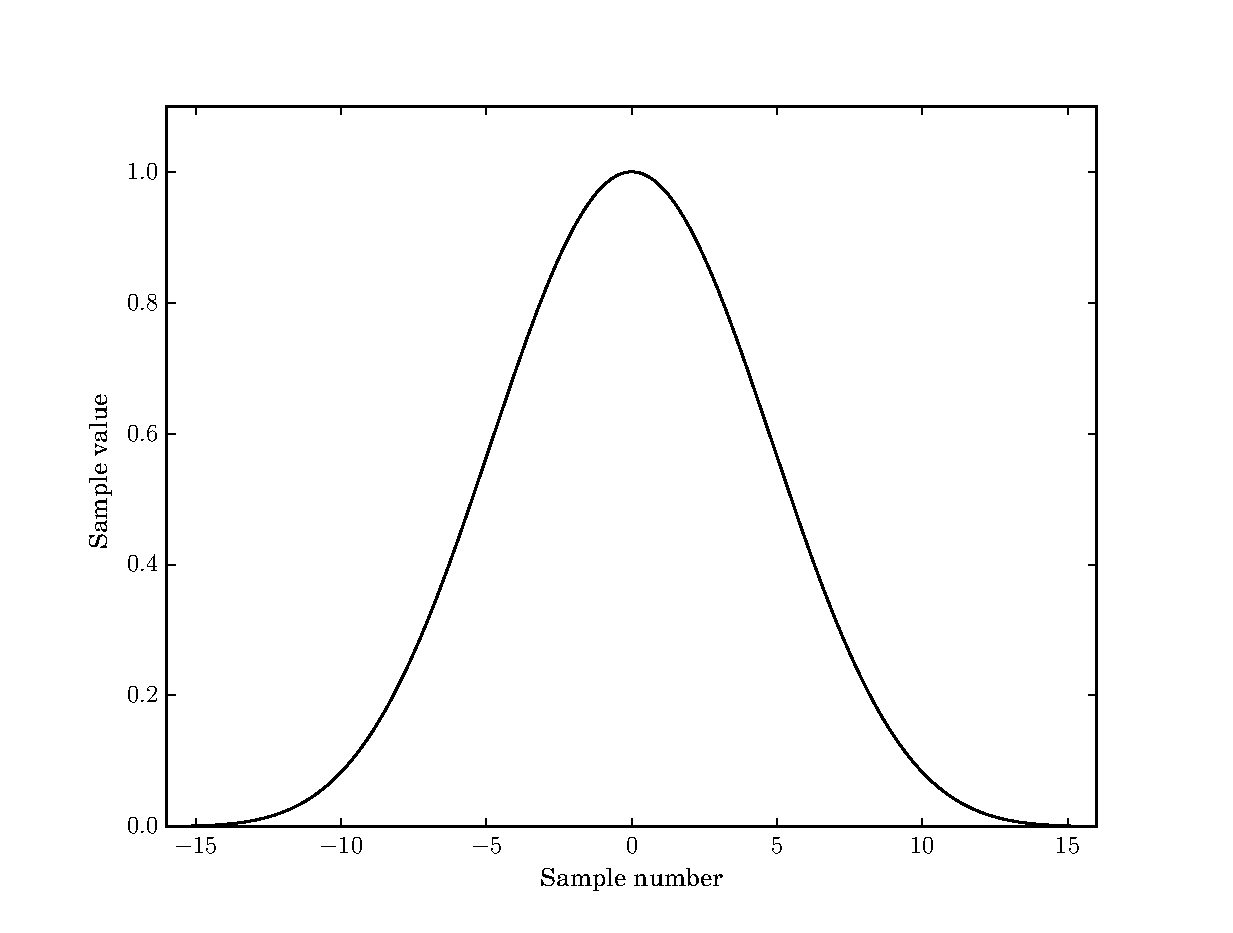
\includegraphics[width=\textwidth]{plots/c1_blackman_td.eps}
\end{figure}

\begin{figure}
    \caption{}
    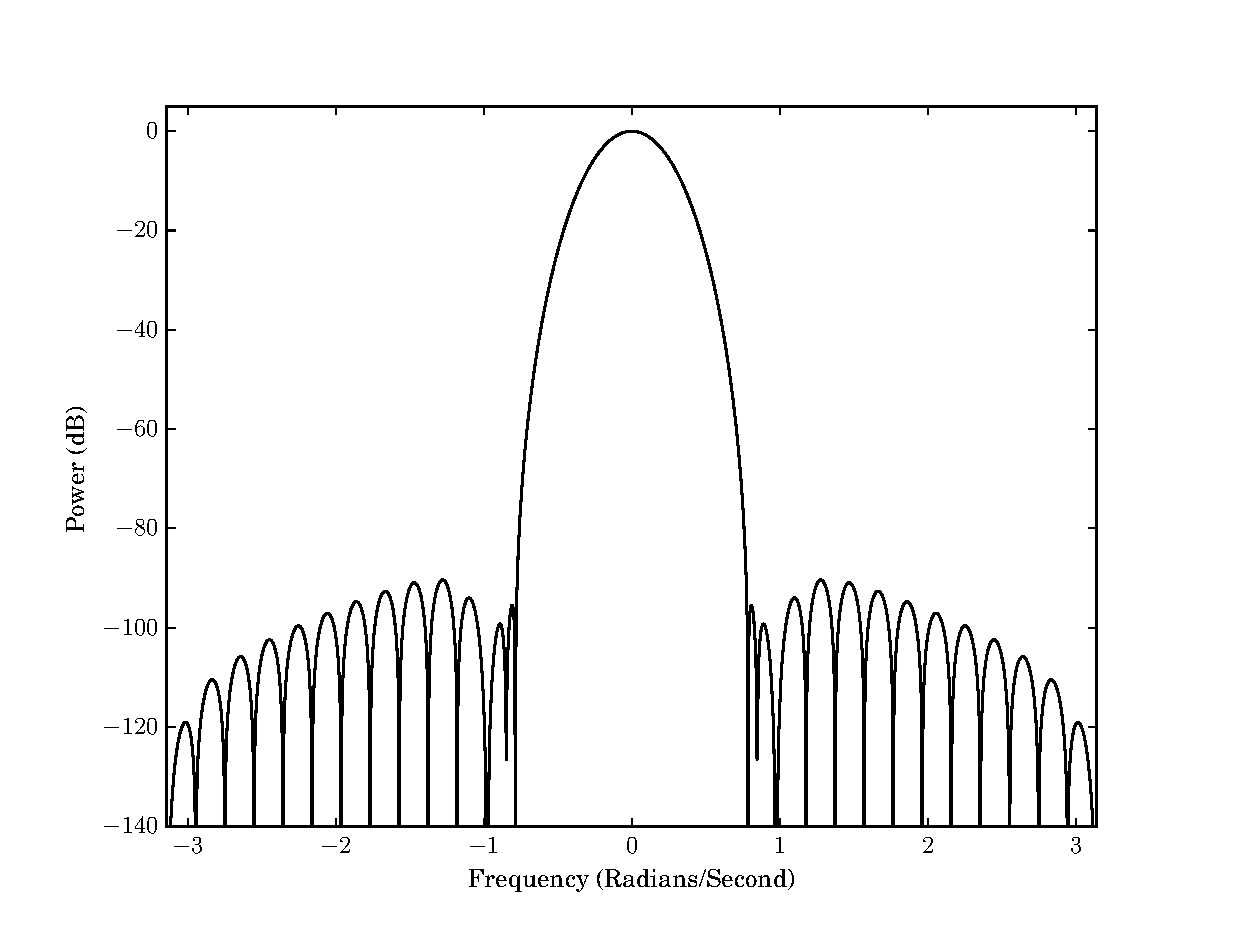
\includegraphics[width=\textwidth]{plots/c1_blackman_fd.eps}
\end{figure}

\bibliographystyle{plain}
\bibliography{thesis}
\end{document}
